\documentclass{article}
\usepackage[utf8]{inputenc}
\usepackage{amsmath}
% \usepackage[linesnumbered,ruled,vlined]{algorithm2e}
% \usepackage{algorithmic}
\usepackage{cleveref}
\usepackage{titling}
\usepackage{flexisym}
\usepackage{enumitem}
\usepackage{color}
\usepackage{graphicx}
\usepackage{booktabs}
\usepackage{array}
\usepackage[paper=a4paper,margin=1in]{geometry}
\usepackage{scalerel,amssymb}
\usepackage{algorithm}
\usepackage{algpseudocode}
\usepackage{caption}
\usepackage{subcaption}
\usepackage{listings}
\usepackage{xspace}
\lstset{
  backgroundcolor=\color{backcolour},   
  commentstyle=\color{codegreen},
  keywordstyle=\color{magenta},
  language = Prolog,
  literate = {-}{-}1,
  breaklines=true, 
  numbers=left,
  basicstyle=\sffamily,
  %keywordstyle=\bfseries,
  %morekeywords={reached,  in, source, sink,edge,node},
}
\usepackage{xcolor}
\definecolor{codegreen}{rgb}{0,0.6,0}
\definecolor{codegray}{rgb}{0.5,0.5,0.5}
\definecolor{codepurple}{rgb}{0.58,0,0.82}
\definecolor{backcolour}{rgb}{0.95,0.95,0.92}
\usepackage{tikz}
\usepackage{scalerel,amssymb}
\usetikzlibrary{positioning, fit, calc, shapes.geometric}
\tikzset{block/.style={draw, thick, text width=2cm , minimum height=1.3cm, align=center},   
line/.style={-latex}     
} 
\algnewcommand\algorithmicforeach{\textbf{for each}}
\algdef{S}[FOR]{ForEach}[1]{\algorithmicforeach\ #1\ \algorithmicdo}
\def\mcirc{\mathbin{\scalerel*{\circ}{j}}}
\def\msquare{\mathord{\scalerel*{\Box}{gX}}}
\newtheorem{theorem}{Theorem}
\newtheorem{proposition}{Proposition}
\newtheorem{lemma}{Lemma}
\newtheorem{example}{Example}
\newtheorem{definition}{Definition}
\newtheorem{remark}{Remark}
\newtheorem{proof}{Proof}
\newcommand{\m}{\mathcal{M}}
\newcommand{\mzero}{\mathcal{M}_0}
\newcommand{\mone}{\mathcal{M}_1}
%% commands for submission 
\newcommand{\unsat}{\ensuremath{\mathsf{unsat}}}
\newcommand{\pos}[1]{\ensuremath{\mathsf{pos}(#1)}}
\newcommand{\ngt}[1]{\ensuremath{\mathsf{neg}(#1)}}
\newcommand{\cls}[1]{\ensuremath{\mathsf{c}(#1)}}
\newcommand{\vrbl}[1]{\ensuremath{\mathsf{v}(#1)}}
\newcommand{\program}[1]{\mathcal{P}(#1)}
\newcommand{\body}[1]{\mathsf{Body}(#1)}
\newcommand{\true}{\ensuremath{\mathsf{true}}\xspace}
\newcommand{\false}{\ensuremath{\mathsf{false}}\xspace}
\newcommand{\copyatom}[1]{#1\textprime}
\newcommand{\mmodel}[1]{\mathsf{MM}(#1)}
\newcommand{\Card}[1]{|#1|}
\newcommand{\Var}[1]{\mathsf{Var}(#1)}
%% upto now
\newcommand{\minimal}[1]{\mathsf{MM}(#1)}
\newcommand{\answer}[1]{\mathsf{AS}(#1)}
\title{Weekly Report}
\begin{document}
\date{13 March 2024}
\section{Methodology}
In this section, for a given Boolean formula $F$, we introduce an ASP program where each answer set of the program correspondences to the unsatisfiable cores of $F$.
Finally, we introduce some optimization techniques to improve computational efficiency.  
\subsection{ASP Encoding}
For a given Boolean formula $F$, we introduce an ASP program $\program{F}$.
The ASP program $\program{F}$ involves introducing some ASP atoms as follows:
\begin{itemize}
  \item $\cls{i}$: for each clause $C_i \in F$, we introduce a free or choice atom $\cls{i}$
  
  The choice atom $\cls{i}$ indicates that the corresponding clause $C_i$ is under consideration. 
  \item $\pos{x}$, $\ngt{x}$: for each variable $x \in \Var{F}$. 
  
  We adapt the following symbolic interpretations: $\pos{x}$ ($\ngt{x}$ resp.) interprets that variable $x$ is assigned to \true (\false resp.). While 
  a variable cannot be assigned both values simultaneously, in our program $\program{F}$, it is likely that some its interpretations contains both $\pos{x}$ and $\neg{x}$ simultaneously. 
  \item $\unsat$: we introduce an atom $\unsat$ to denote that at least one of the under consideration clauses is unsatisfied.
\end{itemize}
\begin{lstlisting}[caption={Program $\program{F}$},label={code:as_to_uc},captionpos=b,mathescape=true,escapechar=|,float]
  % for each variable $x \in X$
  $\pos{x} \vee \ngt{x}$.|\label{line:each_variable}|
  % for each clause $C_i = x_1 \vee \ldots x_{k}, \vee \neg{x_{k+1}} \vee \ldots \neg{x_{k+m}}$
  $\unsat \leftarrow \cls{i}, \ngt{x_1}, \ldots \ngt{x_k}, \pos{x_{k+1}}, \ldots \pos{x_{k+m}}$.|\label{line:reach1}|
  % at least one clause must be falsified
  $\leftarrow$ not $\unsat$.|\label{line:unsat}|
  % for each variable X
  $\pos{x} \leftarrow \unsat$.
  $\ngt{x} \leftarrow \unsat$.
  % for each clause $C_i$, there is one free variable
  $\{ \cls{i} \}.$
\end{lstlisting}
\begin{lstlisting}[caption={Reduct of $\program{F}$ w.r.t. $M$},label={code:program_to_reduct},captionpos=b,mathescape=true,escapechar=|,float]
  % for each variable $x \in X$
  $\pos{x} \vee \ngt{x}$|\label{line:each_variable}|
  % for each clause $C_i \in M$
  $\unsat \vee \neg \cls{i} \vee \neg \ngt{x_1} \vee \ldots \vee \neg \ngt{x_k} \vee \neg \pos{x_{k+1}} \vee \ldots \vee \neg \pos{x_{k+m}}$|\label{line:reach1}|
  % for each variable X
  $\pos{x} \vee \neg \unsat$
  $\ngt{x} \vee \neg \unsat$
  % for each clause $c_i \in M$
  $\cls{i}$
\end{lstlisting}
Among the atoms of $\program{F}$, the atom $\cls{i}$ correspondences to clause $C_i \in F$. 
An interpretation $M$ over the atoms of $\program{F}$ considers a set of clauses of $F$.
More specifically, if $\cls{i} \in M$ then clause $C_i$ is considered by interpretation $M$.
We use the notation $M_{\downarrow \cls{.}}$ to denote the considered clauses under an interpretation. 
With the above set of atoms, given a Boolean formula $F = \bigwedge_{i=1}^{n} C_i$, we introduce an ASP program $\program{F}$ such that each of the unsatisfiable cores of $F$ one-to-one corresponds to answer sets of $\program{F}$. 
The ASP program $\program{F}$ is introduced in Listings~\ref{code:as_to_uc}. 
Moreover, we analyze the reduct of $\program{F}$, which is important for the theoretical analysis of the encoding. 


The theoretical guarantee of the program is established in~\Cref{lemma:as_to_uc_proof}.
\begin{lemma}
  \label{lemma:as_to_uc_proof}
  Each answer set $\sigma \in \answer{\program{F}}$ one-to-one corresponds to an unsatisfiable core of $F$.
\end{lemma}
\begin{proof}
  The lemma has two parts to proof:
  \begin{enumerate}
    \item For each $\sigma \in \answer{\program{F}}$, $\sigma_{\downarrow \cls{.}}$ corresponds to an unsatisfiable core of $F$
    \item Each unsatisfiable core $U$ of $F$ corresponds to an answer set of $\program{F}$ 
  \end{enumerate}
  Proof of `Part $1$': For an answer set $\sigma \in \answer{\program{F}}$, let assume $\sigma_{\downarrow c/1} = \{c_{i_1}, \ldots, c_{i_k}\}$.
  We proof that the clause set of $\sigma_{\downarrow c/1}$ constitutes an unsatisfiable core of $F$.

  Under answer set semantics, $\unsat \in \sigma$ (line~\ref{line:unsat} of encoding~\ref{code:as_to_uc}) and $\forall x \in \Var{F}$, $\{\pos{x}, \ngt{x}\} \subset \sigma$.
  Under clark completion semantics, since $\unsat \in \sigma$, $\exists r \in \program{F}$ such that 
  $\body{r}$ is evaluated to $\true$, which follows that there is a clause $C_i$ such that 
  $\cls{i} \in \sigma$ and for each $x \in c_i$, $\ngt{x} \in \sigma$ and $\neg{x} \in c_i$, $\pos{x} \in \sigma$.
  Note that $\forall x \in \Var{F}$, $\{\pos{x}, \ngt{x}\} \subset \sigma$, which interprets that each variable is assigned to both \true and \false.
  It follows that within the set of clause $\sigma_{\downarrow c/1}$, the clause $c_i$ is not satisfied even after assigning each variable to both \true and \false. 
  Thus, the clause set $\sigma_{\downarrow \cls{.}}$ constitutes a unsatisfiable core of $F$.

  Proof of `Part $2$': Let assume that the clause set $U = \{c_1, \ldots c_n\}$ is a unsatisfiable core of $F$.
  We proof that the clause set $U$ corresponds to an answer set of $\program{F}$. We show that given $U = \{c_{i_1}, \ldots c_{i_n}\}$, 
  $\sigma = \{\cls{i_1}, \ldots, \cls{i_n}\} \cup \{\unsat\} \cup \{\pos{x}, \ngt{x}| \forall x \in \Var{F}\}$ is an answer set of $\program{F}$.
  
  It is trivial to show that $\sigma \models \program{F}$. We show that  $\sigma$ is a minimal model of $\program{F}^{\sigma}$ by showing that each atom of $\sigma$ is justified in $\program{F}^{\sigma}$. 
  The $\program{F}^{\sigma}$ is a propositional encoding~\ref{code:program_to_reduct}.
  Since $\unsat \in \sigma$, there is no clause corresponding to the rule in line~\ref{line:unsat}. 
  Note that since $U$ is an unsatisfiable core of $F$, there exists a clause $C_{i_k} \in U$, $k \in [1,n]$ such that $C_{i_k}$ is not satisfied.
  Following the particular clause of $\program{F}^{\sigma}$, which contains the literal $\neg \cls{i_k}$, the atom $\unsat$ is justified. 
  Moreover, $\unsat \in \sigma$ implies that $\forall x \in \Var{F}$, both $\pos{x}$ and $\ngt{x}$ are also justified.
  Since each atom within $\sigma$ is justified, $\sigma$ is a minimal model of $\program{F}^{\sigma}$. It completes the proof. 
\end{proof}
\section{New MUS Solver using Clingo}
\section{Computing MUSes~\cite{LPMM2016} via Answer Set Programming}
\paragraph{Variables:}
\begin{itemize}
    \item For each clause $c$, introduce a variable $d(c)$
    \item For each variable $x$, introduce two variables $p(x)$ and $n(x)$
\end{itemize}
\paragraph{Rules:}
\begin{itemize}
    \item for each clause $\neg{\ell_1} \vee \ldots \vee 
    \neg{\ell_k} \vee \ell_{k+1} \vee \ldots \vee \ell_{k+m}$, 
    introduce a rule as follows:\\
    $u \leftarrow n(\ell_1), \ldots, n(\ell_k), p(\ell_{k+1}), p(\ell_{k+m}), d(c)$\\
    $u$ is true denotes that at least one of the clauses is satisfied.
    \item add a rule: $\leftarrow \textsf{not } u.$,
    which means that at least one of the clauses is unsatisfiable
    \item for each variable $x$, add a disjunctive rule: $p(x) ; n(x).$\\
    which denotes that each variable must be assigned to at least one of the values.
    \item for each variable $x$, add two rules: $p(x) \leftarrow u$ and $n(x) \leftarrow u$\\
    which denotes at least one of the clauses is UNSAT even after trying out all possible combinations of variables.
\end{itemize}
\paragraph{One-to-one correspondence between MUS and answer sets.}
Each of the $d(i)$-subset minimal models of the ASP program is a MUS of the original formula. 
\paragraph{Experimental Results}
\begin{table}[h]
  \centering
  \begin{tabular}{m{5em} m{5em} m{6em} m{10em}} 
  \toprule
  % & & \rotatebox{60}{\clingo} & \rotatebox{60}{DynASP} & \rotatebox{60}{Ganak}  & \rotatebox{60}{ApproxMC} & \rotatebox{60}{ApproxASP} \\ 
   & marco & unimus & Clingo\\
  \midrule
  %6491 & 6379 & 7743 & 5183 & 6094 & 5599\\
  \#Solved & 264 & 268 & 656\\
  \midrule
  PAR-$2$ & 5501 & 5480 & 2928\\
  \bottomrule
  \end{tabular}
  \caption{The performance of different MUS solvers.}
  \label{table:mus_counting_result}
\end{table}

\begin{figure}
  \centering
  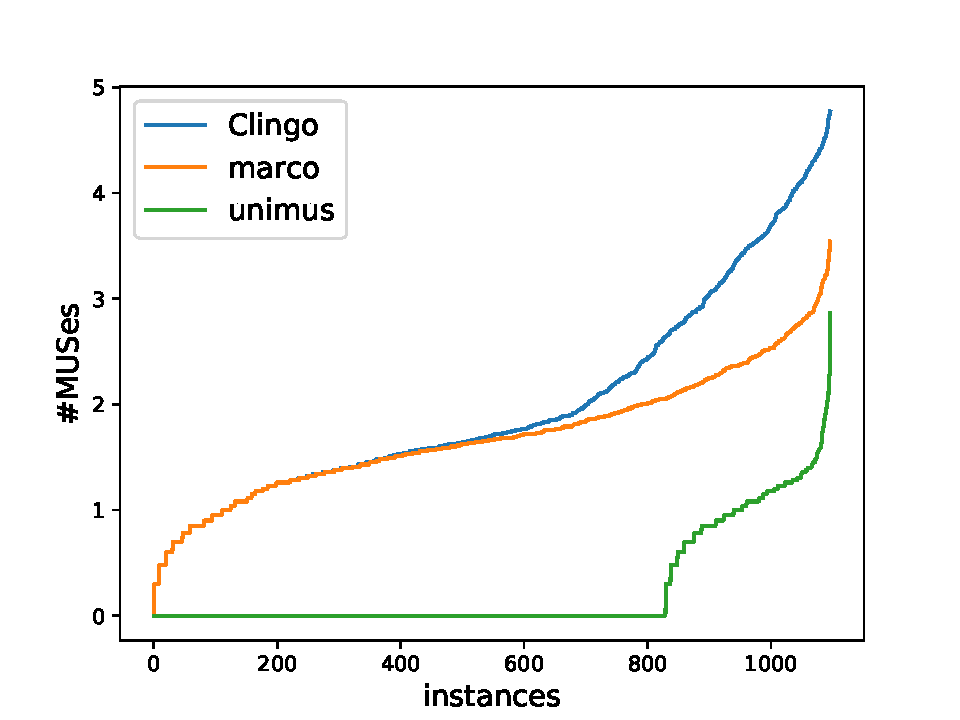
\includegraphics[scale=0.5]{images/countMUS.pdf}
  \caption{The number of enumerated MUSes by different MUS solvers.}
\end{figure}


\newpage
\section{Computing MUSes~\cite{LPMM2016} via Answer Set Programming}
\paragraph{Variables:}
\begin{itemize}
    \item For each clause $c$, introduce a variable $d(c)$
    \item For each variable $x$, introduce two variables $p(x)$ and $n(x)$
\end{itemize}
\paragraph{Rules:}
\begin{itemize}
    \item for each clause $\neg{\ell_1} \vee \ldots \vee 
    \neg{\ell_k} \vee \ell_{k+1} \vee \ldots \vee \ell_{k+m}$, 
    introduce a rule as follows:\\
    $u \leftarrow n(\ell_1), \ldots, n(\ell_k), p(\ell_{k+1}), p(\ell_{k+m}), d(c)$\\
    $u$ is true denotes that at least one of the clauses is satisfied.
    \item add a rule: $\leftarrow \textsf{not } u.$,
    which means that at least one of the clauses is unsatisfiable
    \item for each variable $x$, add a disjunctive rule: $p(x) ; n(x).$\\
    which denotes that each variable must be assigned to at least one of the values.
    \item for each variable $x$, add two rules: $p(x) \leftarrow u$ and $n(x) \leftarrow u$\\
    which denotes at least one of the clauses is UNSAT even after trying out all possible combinations of variables.
\end{itemize}
\paragraph{One-to-one correspondence between MUS and answer sets.}
Each of the $d(i)$-subset minimal models of the ASP program is a MUS of the original formula. 


\bibliography{main} 
\bibliographystyle{apalike}
\end{document}




